\chapter{Laplace's method}
We will calculate the asymptotic to the Gamma function -- Sterling formula\footnote{First calculated by de Moivre, but Sterling contributed by calculating a certain pre-factor.}.\\
\ \newline 
For \emph{sharply peaked integrands} where the dominant contribution to the integral comes from the neighbourhood of a single point. As some parameter $x$ becomes large, the ``bell-shaped'' integrand becomes narrower, giving a much better approximation.

\paragraph{Example 1:} Take the integral
\begin{align*}
	I(x) = \int_{-10}^{10} \me^{-xt^2} \md t \qquad x \rightarrow \infty
\end{align*}
Note the limit which are not from $-\infty$ to $\infty$ which is a known integral (can be done exactly).  This is a Laplace style integral discussed in the previous lecture with $f(t)=1$ and $\phi(t) = -t^2$. Integration by parts breaks down since $\phi'(t)=0$ in the domain of integration. Anyway, as we shall see, we get an expansion in \emph{fractional} powers of $x$ (not integer powers), which means the Laplace method would not have worked. Now a very crude estimate of this integral is the area under the curve which is simply the height ($=1$) times the width (where the integrand drops to $1/e$ of its peak value)
\begin{align*}
	I(x) \sim O\left({1}/{\sqrt{x}}\right)
\end{align*}
The scaling as we shall see is right, but we are missing a prefactor which we next determine. The region where $ |t| \gg 1/\sqrt{x} $ contributes exponentially small terms (TST) which will not affect the asymptotics (``subdominant'' to $I(x)$). This allows us to add/subtract them!
\begin{align*}
	I(x) &= \int_{-10}^{10} \me^{-xt^2} \md t \\
	&= \int_{-\infty}^{\infty} \me^{-xt^2} \md t + \mathrm{TST} \\
	& \sim \sqrt{\frac{\pi}{x}}
\end{align*} 
To check that the remainder terms are indeed TST, observe
\begin{align*}
	\int_{-10}^{10}() = \int_{-\infty}^{\infty}() - 2 \underbrace{\int_{10}^{\infty} ()}_{\text{bound ?}}
\end{align*}
To find the bounds on the above integral, note that for $t > 10$, the parabola $t^2$ always lies above the straight line $10t$ and therefore for positive $x$
\begin{align*}
	\int_{10}^{\infty}\me^{-xt^2} \md t &< \int_{10}^{\infty}\me^{-10xt} \md t = \left. \frac{\me^{-10xt}}{-10x}\right|^\infty_{10} \\
	&< \frac{1}{10x} \me^{-100x} \ll O\left(\frac{1}{\sqrt{x}}\right)
\end{align*}

\paragraph{Example 2:} Consider
\begin{align*}
	I(x) = \int_{-\infty}^{\infty} \me^{-x \cosh t} \md t
\end{align*}
The function $\cosh t$ is itself like a parabola which is growing exponentially rather than quadratically. Now for small $t$
\begin{gather}
	\cosh t \approx 1 + \frac{t^2}{2!} \label{eqn:cosht}
\end{gather}
so the integrand is like a bell-shaped curve, except now the height is order $\me^{-x}$. So as $x$ becomes large, the integrand becomes narrower and lower. To the leading order, it is OK to approximate $\cosh t$ using eqn. \ref{eqn:cosht} in the neighbourhood of its maximum as $t \rightarrow 0$. Of course when $t$ is large, our approximation is pretty bad, but it does not matter since that part of the integration is contributing TST anyway (for large $x$)! 
\begin{align*}
	I(x) &\sim \me^{-x}\int_{-\infty}^{\infty} \me^{-xt^2/2} \md t \\
	& \sim \sqrt{\frac{2\pi}{x}} \me^{-x}
\end{align*}
But we can go higher order: eqn. \ref{eqn:cosht} motivates an exact change of variable such that
\begin{gather*}
	\cosh t = 1 + \tau^2
\end{gather*}
Since Gaussian integrals are helpful, we make sure we get one by defining the new variable in the above manner and solve this $\tau$ integral.
\begin{align*}
	I(x) = \sqrt{2}\me^{-x} \int_{-\infty}^{\infty} \frac{1}{\sqrt{1+\frac{1}{2}\tau^2}}\me^{-x \tau^2} \md \tau
\end{align*} 
Worth noting that at the lower and upper limits, we are faced with a choice of sign. We pick $\tau = \pm \infty$ corresponding to $t = \pm \infty$ (distortion of $t$ axis). We may also take twice the area under the curve from $t=0$ to $\infty$ and that also helps us select the limits $\tau=0$ to $\infty$.\\
\ \newline 
Now as $x \rightarrow \infty$, we see that $\me^{-x \tau^2}$ gets more sharply peaked about $\tau=0$ and we can Taylor expand the function in the denominator about this point. Note that the MacLaurin series
\begin{gather*}
	(1+\tau^2/2)^{-1/2} = 1 - \frac{\tau^2}{4} + \frac{3}{32} \tau^4 - \dots 
\end{gather*}
converges iff $|\tau^2/2|<1$, i.e. $-\sqrt{2}<\tau <\sqrt{2}$. However, the integral over the domain $-\infty < \tau < \infty$ is justified since the region outside the convergence interval would only contribute TST\footnote{These steps are along the lines of the ``Watson Lemma''.} (expansion diverges but does no harm).
\begin{align*}
	I(x) &\sim \sqrt{2}\me^{-x} \int_{-\infty}^{\infty} \me^{-x \tau^2} \left(1 - \frac{\tau^2}{4} + \frac{3}{32}\tau^4-\dots \right) \md t \\
	& \sim \sqrt{\frac{2\pi}{x}}\me^{-x} \left(1 - \frac{1}{8x} + \frac{9}{128x^2}-\dots \right)
\end{align*}
To evaluate the Gaussian integrals, we use the well known result
\begin{gather*}
	\int_{-\infty}^{\infty} \me^{-xt^2} \md t = \sqrt{\frac{\pi}{x}}
\end{gather*}
and apply repeated differentiation with respect to the parameter $x$ to derive 
\begin{align}
	\int_{-\infty}^{\infty} \me^{-xt^2} t^{2n} \md t &= \sqrt{\pi}(-1)^n \frac{\pd}{\pd x^n} x^{-\frac{1}{2}} \\
	&= \sqrt{\frac{\pi}{x}} \frac{(2n-1)!!}{(2x)^n} \nonumber 
\end{align}

\paragraph{Example 3:} The Stirling formula for $\Gamma(x+1)=x!$ as $x \rightarrow \infty$
\begin{gather*}
	\Gamma(x+1) = \int_{0}^{\infty} t^x \me^{-t} \md t
\end{gather*}
Not obvious where this integral sharply peaks or in fact has a peak as $x \rightarrow \infty$. The \emph{first} trick is a slight rearrangement to express the function as
\begin{align*}
	\Gamma(x+1) = \int_{0}^{\infty} \me^{x \ln t} \me^{-t} \md t
\end{align*}
The strategy for such Laplace-type integrals is to find where the exponential peaks and expand about the point. So we proceed to determine the point where the exponential is maximized, i.e. where $x \ln t - t$ has a maxima. Therefore the bell is centered about $t=x$, which itself is moving to infinity (movable maxima). \\
\ \newline
In such problems it is always good to pick a coordinate such that the peak is not moving. We make the substitution
\begin{gather*}
	s = \frac{t}{x}
\end{gather*}
which has the advantage that the maxima is now at $s=1$ for all $x$. This is the \emph{second} trick. With this change
\begin{align}
	\Gamma(x+1) = x^{x+1} \int_{0}^{\infty} \me^{x (\ln s - s)} \md s \label{eqn:Gamma-fixed-peak}
\end{align}
The \emph{third} trick is to expand the term $\ln s - s$ about its maximum at $s=1$ (see Fig. \ref{fig:strogatz-wk04}). The Taylor expansion reads
\begin{align}\label{eqn:Gamma-Taylor}
	\ln s -s = - \left[1+ \frac{(s-1)^2}{2} \dots \right]
\end{align}
The integral simplifies to
\begin{align*}
	\Gamma(x+1) \sim x^{x+1} \me^{-x} \int_{0}^{\infty} \me^{-x\frac{(s-1)^2}{2}} \md s
\end{align*}
The \emph{fourth} trick is to add the tails that contribute TST and expand the lower limit of the integral from 0 to $-\infty$. This readily yields
\begin{align}\label{eqn:stirling-approx}
	\Gamma(x+1) \sim \sqrt{\frac{2\pi}{x}}x^{x+1}\me^{-x}
\end{align}
which for integers provides the well know identity
\begin{gather}
	n! \sim \sqrt{2\pi n} \left(\frac{n}{e}\right)^n
\end{gather}
The above is a one-term Stirling approximation to the Gamma integral. If we want to get higher order correction terms, we take eqn. \ref{eqn:Gamma-fixed-peak} and, inspired by eqn. \ref{eqn:Gamma-Taylor}, perform the exact change of variable
\begin{align*}
	\ln s - s = 1 + \tau^2
\end{align*}
This converts the exponential term to an exact Gaussian and allows us to expand the newly introduced prefactor algebraically (cf. previous example).  

\begin{figure}[!h]
	\centering
	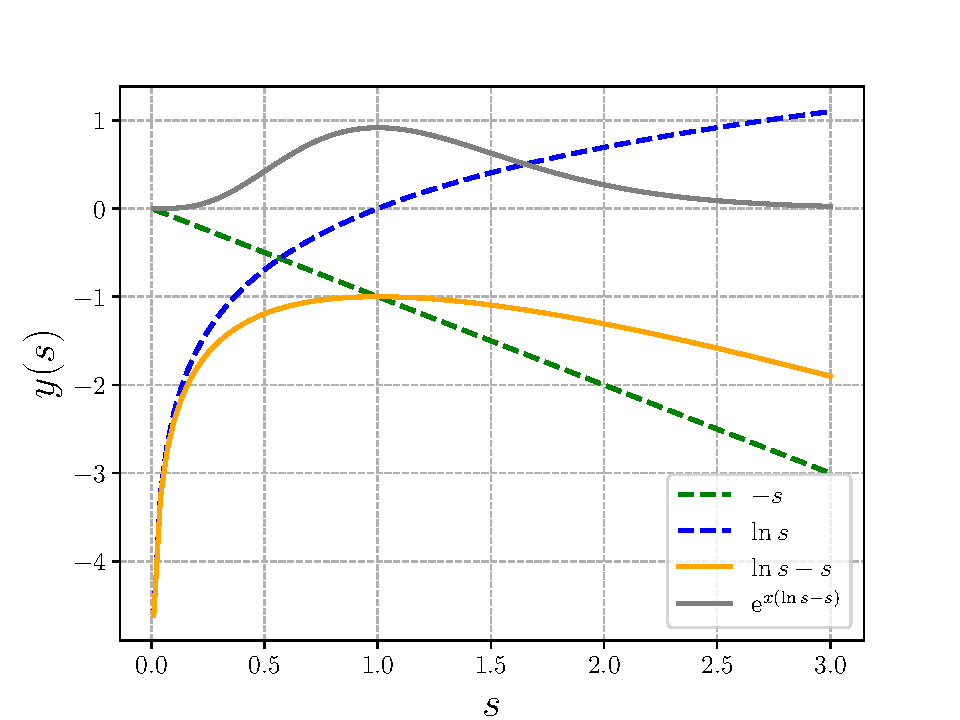
\includegraphics[width=0.75\textwidth]{./plots/pdf/strogatz-wk04.pdf}
	\caption{Plotting the integrand (gray) in the integral given by eqn. \ref{eqn:Gamma-fixed-peak}. This is scaled by a multiplicative factor for visualization. For very large values of $s$ the linear term dominates, whereas for $s \rightarrow 0$ the logarithmic term is dominant.}
	\label{fig:strogatz-wk04}
\end{figure}

{\color{red}[To do]}
\begin{itemize}
	\item Higher order expansion... 
\end{itemize}


